\documentclass{article}
\addtolength{\oddsidemargin}{-.875in}
\addtolength{\evensidemargin}{-.875in}
\addtolength{\textwidth}{1.75in}
\addtolength{\topmargin}{-1.0in}
\addtolength{\textheight}{1.80in}
\usepackage{hyperref}
\usepackage{wrapfig}
\usepackage{sidecap}
\usepackage[pdftex]{graphicx}
\usepackage[utf8]{inputenc}
\usepackage[spanish]{babel}
\begin{document}
\pagestyle{empty}
\noindent

\noindent
{\sc Parcial \#2  - Física II (2017-10)---Profesor: Jaime Forero--- 19
  de Abril de 2017}  
\\
NOTA: Todas las respuestas deben tener una justificaci\'on f\'isica y
matem\'atica de acuerdo a los temas vistos en el curso. Se permite el
uso de calculadora.\\
\\
% Cap 22 Ley de Gauss
Problema 1. (20 puntos).\\
Considere una esfera gelatinosa de radio R con una carga total 2Q 
distribu\'ida de manera homog\'enea en todo su volumen.
Adentro de esta esfera se encuentran dos cargas puntuales que se
pueden desplazar dentro de la esfera, cada una con carga -Q. Ver la
Figura.
Las cargas se encuentran sobre una l\'inea que pasa por el centro de la
esfera.
Calcule la  distancia $a$ que debe haber entre estas dos cargas
puntuales para que el sistema se encuentre en equilibrio.
Exprese su respuesta en t\'erminos de R, Q y $\epsilon_0$.\\
%
% Cap 23 Potencial Electrico
Problema 2 (20 puntos) \\
Una esfera maciza conductora de radio $10$cm est\'a cargada y se
mantiene fija sobre una mesa.
El campo el\'ectrico en su superficie es de $2000$ N/C.
Arriba de esta esfera, muy cerca a su superficie, hay una carga positiva de
$10^{-9}$C y masa $10^{-6}$ kg que se mantiene inicialmente en reposo
por una fuerza externa.
Cuando esta fuerza deja de actuar, la peque\~na carga va a ser
repelida por la esfera.
Encuentre la velocidad en m/s que tendr\'a la peque\~na carga cuando
se encuentre a una distancia de $10$ m de la la esfera. Desprecie la
fuerza de gravedad.\\ 
%
% Cap 24 Capacitores y Capacitancia
Problema 3 (20 puntos)\\
Entre las placas de un condensador de area $A$, separaci\'on $d$ y
densidades superficiales de carga $\sigma$ se ubica un conductor de
grosor $a$ tal como muestra la Figura. Encuentra la capacitancia en
t\'erminos de $A$, $d$ y $a$.\\
%
% Cap 25 Resistencia y Resistividad
Problema 4 (20 puntos)\\
Se tiene un tri\'angulo de resistencias como muestra la
Figura. $R_1=10\Omega$, $R_2=5\Omega$ y $R_3=100\Omega$. Encuentre la
corriente que circula por cada una de las resistencias si se conecta
una fuente de $100$V a los extremos de $R_1$.\\
%
% Cap 26 Reglas de Kirchhoff
Problema 5 (20 puntos)\\
Utilizando las reglas de Kirchhoff encuentre las seis 
corrientes del circuito mostrado en la Figura.
\footnote{Problema tomado de: \url{https://wikieymfi.wikispaces.com/Cicuito+13}.}\\
%
% 6 Bono (Circuitos)
Problema 6 (20 puntos)\\
Encuentre la resistencia equivalente entre los puntos $a$ y $b$
del cubo mostrado en la Figura. Todas
las resistencias en el cubo valen $R$.
  
\begin{wrapfigure}{l}{1.0\textwidth}
\centering
\begin{center}
  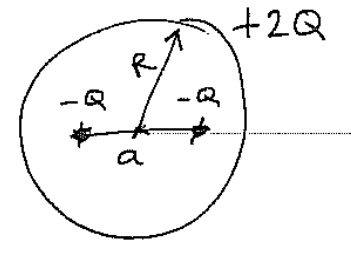
\includegraphics[width=0.30\textwidth]{sphere.png}
  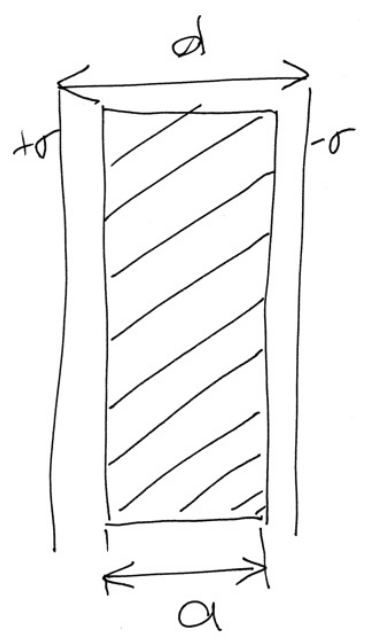
\includegraphics[width=0.15\textwidth]{capacitor.png}
  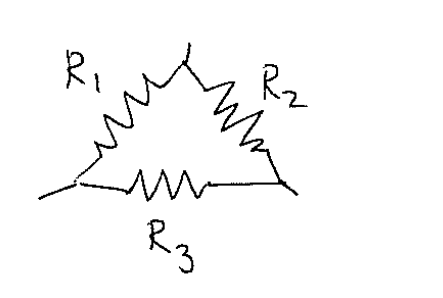
\includegraphics[width=0.30\textwidth]{triangulo.png}
  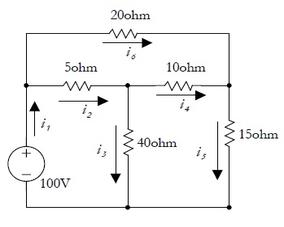
\includegraphics[width=0.30\textwidth]{circuito.jpg}
  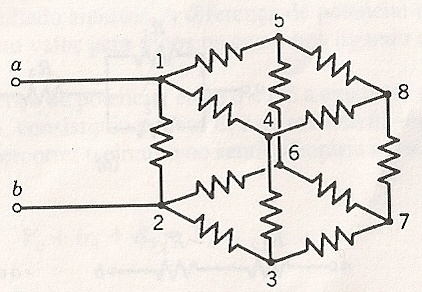
\includegraphics[width=0.30\textwidth]{resistance.jpg}
\end{center}
\caption{Figuras para los ejercicios 1, 3, 4, 5 y 6}
\end{wrapfigure} 



\end{document}
